\refsubsection{Concepts}{subsec:concepts}
\todo{Graphs, eg. concept maps, co-occurrence graphs}
\todo{Classical text representations, eg.tfidf
Categories of algorithms, eg. algorithms on feature vectors, kernelized - algorithms}

\refsubsection{Definitions and Notations}{subsec:definitions_and_notations}
\todo{Lay groundwork for the later description of the problem}
\todo{Introductions to used classifiers, concepts}
\todo{Concretize the problem and its notation}
\todo{Comparison of the used data sources}

\subsubsection{Classification Task}

\subsubsection{Graphs}

\paragraph{Concept Map}
A concept map is a graph where the nodes are concepts.
Concepts are important tokens in a text.
Concepts consist of one or more words.
The directed edges between nodes show that they are related to each other.
Edges can have labels, too.

Concept maps are useful for visualizing concepts and their relation to each other.
Concept maps can be used to quickly explore a given topic and immediately see connections between concepts.
Through the degree of a concept, one can also infer the relative importance of that concept for the underlying text.

By combining different texts of the same topic, one can also create a concept map for that topic - the concepts are not confined to a single text in this case.
The visualization with concept maps of one or more individual texts therefor enables the non-linear exploration of a topic.

\todo{"Capture important concepts and the structure of texts (spanning over whole text)"}
\todo{Creation of concept maps via library by Tobias}

\begin{figure}[h]
\centering
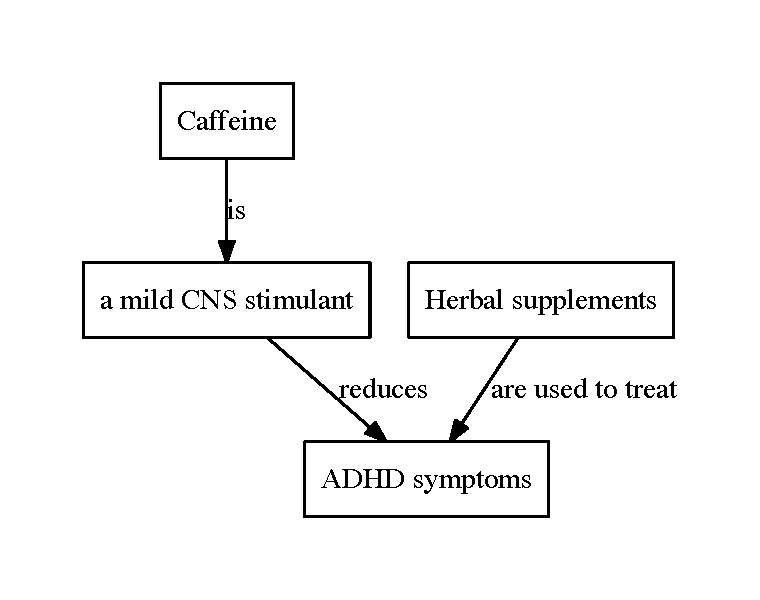
\includegraphics[width=0.5\linewidth]{assets/figures/concept_map.pdf}
\caption{Example of a concept map}
\label{fig:concept_map}
\end{figure}

\paragraph{Co-Occurrence Graph}
A co-occurrence graph, or graph-of-words, is generated from a text by creating a graph with the words of the text as nodes.
There is an edge between two nodes if their labels co-occur in the text.
Two words co-occur when the distance between the words in the text is below a given threshold, the window size.

\subsubsection{Graph kernel}

In most cases, texts are of non-fixed size. Finding a fixed-size representation for texts is crucial for classification since most classification algorithms operate on fixed-size vectors.
The same problem appears in graph classification. The number of the nodes or edges is also not fixed.
There are several approaches to enable graph classification, one being so-called graph kernels.

A graph kernel is a function $K$ which returns a measure of similarity between two graphs:
\begin{equation*}
K: G \times G \rightarrow \mathbb{Q}
\end{equation*}
The graph kernel function has to be:
\begin{itemize}
    \item{\textit{symmetric}: $K(G_1, G_2) = K(G_2, G_1)$}
    \item{\textit{positive semi-definite}: \dots}
\end{itemize}

\todo{$K(G_1, G_2) = \langle \phi(G_1), \phi{G_2} \rangle$}

\todo{Categories of graph kernels, eg. random-walk-based, subtree-based}

\paragraph{Gram matrix}
A gram or kernel matrix for a given kernel is a matrix $A$ where the entries are the pairwise similarities of graphs:
\begin{equation*}
    A_{i,j} = K(G_i, G_j)
\end{equation*}
The gram matrix has to be symmetric by definition since the underlying kernel is also symmetric, so $A_{i,j} = A_{j, i}$.
